\documentclass[journal]{IEEEtran}
% \documentclass[journal]{../sty/IEEEtran}
\usepackage{cite}

%% Graphics package
\usepackage[pdftex]{graphicx}
% declare the path(s) where your graphic files are
\graphicspath{{./pdf/}{./jpeg/}{./png/}}
% and their extensions so you won't have to specify these with
% every instance of \includegraphics
\DeclareGraphicsExtensions{.pdf,.jpeg,.png}

%% For code
\usepackage{listings}

\usepackage{array} % Alignment
\usepackage{fixltx2e} % Column fixes
\usepackage{ctable} % Nicer tables
\usepackage[colorlinks=false, pdfborder={0 0 0}]{hyperref}
\usepackage{tikz}
\usetikzlibrary{shapes,arrows,calc}
%% Define some styles
\tikzstyle{block} = [rectangle, draw, fill=blue!20, 
    text width=6em, text centered, rounded corners, minimum height=4em]
\tikzstyle{line} = [draw, -latex']

% correct bad hyphenation here
\hyphenation{op-tical net-works semi-conduc-tor CustomAudioRecorder FilteringComplete}

\usepackage{ucs} %UTF8
\usepackage[utf8x]{inputenc} % Input encoding

\begin{document}

\lstset{frame=lines,
        language=Matlab,
        breaklines=true,
        numbers=left,
        numbersep=1pt,
        basicstyle=\tiny}

\title{PulseAudio and the knife-alien sound processor\\
-- Taking \textsc{Matlab} to the next level}
\author{Patrik~Dahlström (patda293),~\IEEEmembership{Electronic design programme,~Linköping university}}
% The paper headers
\markboth{PulseAudio and the knife-alien sound processor -- Taking \textsc{Matlab} to the next level}{}

\maketitle

\begin{abstract}
The knife-alien sound processing engine is an easy and intuitive tool to manipulate audio streams, but currently lacks satisfactory audio output. This report describes an attempt to use PulseAudio for audio playback. The implementation presented however does not produce smooth and low-latency playback.

The appendix describe how the PulseAudio implementation can be used together with \textsc{Simulink}.
\end{abstract}

\section*{Introduction}
Sound processing is a subject that is as current today as it was 50 years ago. The knife-alien sound processing engine presents an easy and intuitive way to manipulate an audio stream. Filters are easily added and removed, without the need of stopping and starting recording.

However, \textsc{Matlab}s sound output is far too slow to effectively output audio at the same rate as audio is recorded, and the output become choppy. Therefore an external library is used to decrease latency and choppiness: PulseAudio.

This report will describe the various parts of knife-alien that the author was the major contributor to as well as an evaluation of PulseAudio and how well it substitutes \textsc{Matlab}s built-in audio functions.

The appendix contains a chapter on how PulseAudio can be used together with \textsc{Simulink}

\section{knife-alien}
The knife-alien sound processing engine implement a combination of \textsc{Matlab}s events and listeners concept and a linked list of filters.

\subsection{Functional overview}
The filtering process can be described in 5 steps:
\begin{enumerate}
\item An audio source notifies the event NewAudioData
\begin{enumerate}
\item The topmost graph of the GUI present the frequency spectrum of this data.
\item The new audio data is passed to a dummy filter which does not alter the signal.
\end{enumerate}
\item The data progress through all active filters in order, each filter notifying the event FilteringComplete.
\item The FilteringComplete event of the last filter (which also is a dummy filter) triggers the listener callback functions that will save and play the filtered audio, as well as present it in the bottommost graph of the GUI.
\end{enumerate}
See \autoref*{knife-alien overview} for a graphical overview of this process.

\begin{figure} % knife-alien overview
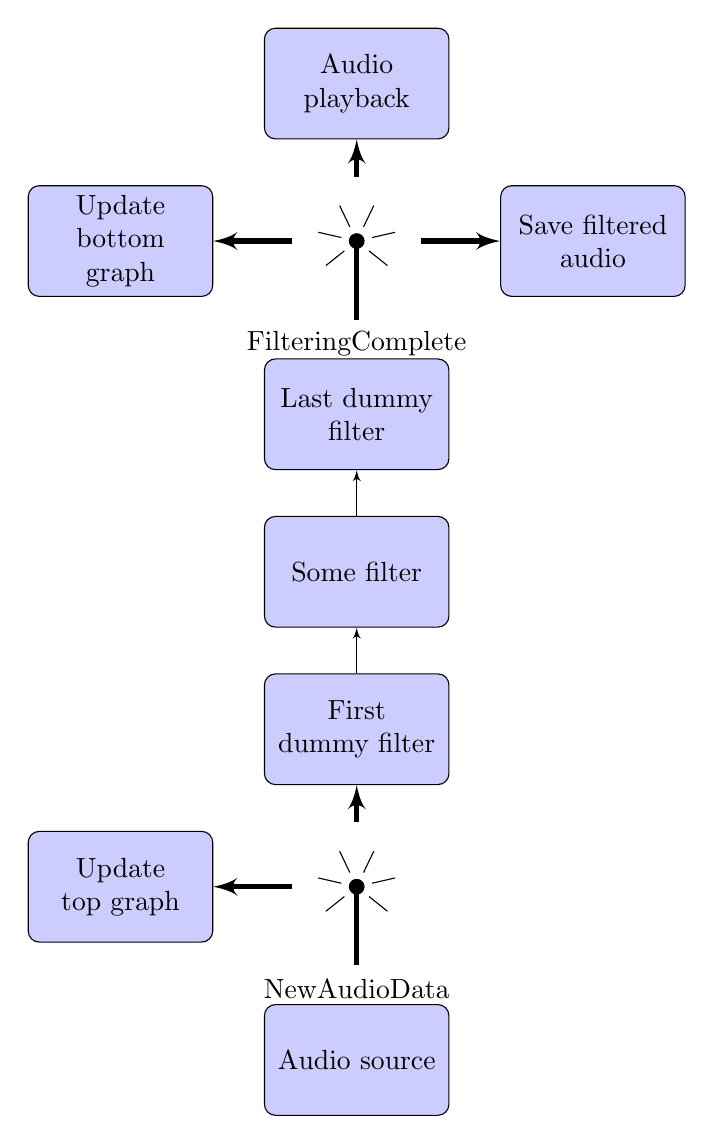
\begin{tikzpicture}[node distance = 2cm, auto]
%% Place nodes
\node [outer sep=7mm] (x) at (0,0) {};
\node [block, below of=x, node distance=2.2cm] (audiosource) {Audio source};
\node [block,above of=x] (firstDummy) {First dummy filter};
\node [block, above of=firstDummy] (filter) {Some filter};
\node [block, above of=filter] (lastDummy) {Last dummy filter};
\node [above of=lastDummy, node distance=2.2cm,outer sep=7mm] (y) {};
\node [block, left of=x, node distance=3cm] (topgraph) {Update top graph};
\node [block, above of=y] (playaudio) {Audio playback};
\node [block, left of=y, node distance=3cm] (bottomgraph) {Update bottom graph};
\node [block, right of=y, node distance=3cm] (saveaudio) {Save filtered audio};

%% Draw broadcast image for NewAudioData
\foreach \x in {1,...,6}{
    \draw (360/7*\x-90:0.2) -- (360/7*\x-90:0.5);
}
\draw[line width=2pt] (0,0) -- (0,-1.0);
\fill (0,0) circle (0.1cm);
\node (newaudiodata) at (0,-1.3) {NewAudioData};

%% Draw broadcast image for FilteringComplete (with some offset hacking)
\foreach \x in {1,...,6}{
    \draw ($(360/7*\x-90:0.2)+(y)$) -- ($(360/7*\x-90:0.5)+(y)$);
}
\draw[line width=2pt] ($(y)$) -- ($(0,-1.0)+(y)$);
\fill ($(0,0)+(y.center)$) circle (0.1cm);
\node (filteringcomplete) at ($(0,-1.3)+(y)$) {FilteringComplete};

%% Draw lines between boxes
\path [line] (firstDummy) -- (filter);
\path [line] (filter) -- (lastDummy);
\path [line, line width=2pt] (x) -- (topgraph);
\path [line, line width=2pt] (x) -- (firstDummy);
\path [line, line width=2pt] (y) -- (bottomgraph);
\path [line, line width=2pt] (y) -- (saveaudio);
\path [line, line width=2pt] (y) -- (playaudio);
\end{tikzpicture}
\caption{Overview of knife alien filtering procedure}
\label{knife-alien overview}
\end{figure}

\subsection{Audio source}
Currently, there are two types of audio sources available in knife-alien: from a microphone or from a wave file\footnote{Currently under development}. The classes responsible for each audio source are \emph{CustomAudioRecorder} and \emph{CustomAudioPlayer} respectively.

All audio sources perform a Fast Fourier Transform on its data before notifying NewAudioData.

For recording audio from a microphone the \textsc{Matlab} class \emph{audiorecorder} was used as base class. \emph{CustomAudioRecorder} adds some properties as well as an event -- NewAudioData.

\textsc{Matlab}s \emph{audiorecorder} class provide the functionality of executing a callback function with regular intervals. This functionality is used by \emph{CustomAudioRecorder} to call its member function customTimerFcn(). 
customTimerFcn() calculates how many new samples have been recorded since last time it was executed and performs a fast Fourier transform on only the new audio data before notifying the NewAudioData event.

The source code of \emph{CustomAudioRecorder} is provided in \autoref*{code:customaudiorecorder}.

\begin{lstlisting}[caption={CustomAudioRecorder.m: Source code of CustomAudioRecorder},
                   label={code:customaudiorecorder}]
classdef CustomAudioRecorder < audiorecorder & handle
    properties
        listener
    end
    properties (SetAccess = protected)
        Data
        Fs
        Nfft
        lastSample
    end
    methods
        function obj = CustomAudioRecorder(Fs,nBits,nChannels)
            obj = obj@audiorecorder(Fs,nBits,nChannels);
            obj.Fs = Fs;
            obj.TimerFcn = @obj.customTimerFcn;
        end
        function customTimerFcn(obj,src,eventData)
            audioData = getaudiodata(src);
            % Update number of samples since last time this function ran
            obj.Nfft = obj.TotalSamples - obj.lastSample;
            obj.lastSample = obj.TotalSamples;
            % Only process last Nfft samples
            audioData = audioData(end-obj.Nfft:end);
            audioData = fft(audioData,obj.Nfft);
            obj.Data = audioData;
            notify(obj,'NewAudioData');
        end
        function reset(obj)
            obj.lastSample = 0;
        end
    end
    methods (Static,Hidden)
        % Overide audiorecorder's private, hidden validateFcn.
        % Had to make this function static, don't really know why.
        function validateFcn(fcn)
        end
    end
    events
        NewAudioData
    end
end
\end{lstlisting}

Documentation for \emph{CustomAudioPlayer} is not contained in this document.

\subsection{Filters}
All filters of the knife-alien sound processing engine are contained in a \textsc{Matlab} package as to separate them from the rest of the knife-alien namespace. This avoids the problem of function name disambiguation with other functions in the knife-alien root tree.

The filters use an abstract superclass called \emph{FilterClass} that defines properties common for all filters. These properties are:
\begin{itemize} % Filter properties
\item Fs – Sample rate
\item UserData – Could be anything
\item Next – A handle to the next filter in a chain of filters
\item Prev – A handle to the previous filter in a chain of filters
\item Data – The actual data
\item Name – A textual representation of the filter
\end{itemize}
These properties are hidden so that they don't show up in the filter configuration box in the main GUI.

\emph{FilterClass} also define an abstract function, filter(), that all subclasses of \emph{FilterClass} have to implement. The only function implemented by \emph{FilterClass} is eventHandler() which acts as wrapper to pass on data to filter().

See \autoref*{code:filterclass} for source code.

\begin{lstlisting}[caption={FilterClass.m: Superclass of all filters},label={code:filterclass}]
classdef (Hidden=true) FilterClass < handle
    properties (Hidden=true)
        Fs
        UserData
        Next
        Prev
    end
    properties (SetAccess = protected,Hidden = true)
        Data
        Name
    end
    methods (Abstract=true)
        filteredData = filter(obj,data)
    end
    methods
        function eventHandler(obj,src,eventData)
            obj.filter(src.Data);
        end
    end
    events
        FilteringComplete
    end
end
\end{lstlisting}

Each filter's implementation of filter() has to call the filter() function of the next filter -- obj.Next.filter() -- for the filtering chain to work. It is also responsible for notifying FilteringComplete although it is not mandatory.

Each filter's constructor is also responsible for populating the Name property.

\subsection{Save filtered data}
Upon creation, knife-alien defines a series of listener callbacks for the FilteringComplete event of the last dummy filter. One of those callback functions is saveFilteredAudio() shown in \autoref*{code:savefilteredaudio}. This function appends data to the file recorded\_audio.wav or creates it if it doesn't exist.

\begin{lstlisting}[caption={saveFilteredAudio.m: Append filtered audio to recorded\_audio.wav},
                   label={code:savefilteredaudio}]
function saveFilteredAudio(obj,eventData)
audioData = ifft(obj.Data);
Y = 0;
if exist('recorded_audio.wav','file')
    Y = wavread('recorded_audio.wav');
end
Y = [Y; audioData];
wavwrite(Y,obj.Fs,'recorded_audio.wav');
\end{lstlisting}

\subsection{Audio playback}
Another listener callback function defined on startup is playFilteredAudio(). When data arrives to this function it is Fourier transformed and of type double. For audio playback this data has to be inversely transformed and converted to int16 to be compatible with the playAudio() function call. Only data of more than 512 samples are played to increase performance.

The UserData property of the last dummy filter contain the address of an C object needed by playAudio(). More on this in \autoref*{sec:pulseaudio}.

\begin{lstlisting}[caption={playFilteredAudio.m: Inverse transform, convert and play data},
                   label={code:playfilteredaudio}]
function playFilteredAudio(obj,eventData)
if numel(obj.Data) > 512
    audioData = int16(ifft(obj.Data)*32767);
    playAudio(obj.UserData,audioData);
end
\end{lstlisting}

\subsection{Update bottom graph}
How the bottom graph is updated is beyond the scope of this document.

\section{PulseAudio}
\label{sec:pulseaudio}
PulseAudio is a sound system for POSIX system, meaning that it is a proxy for sound applications. It is an integral part of several popular Linux distributions and is used by various mobile devices.

PulseAudio is built on a server-client model, in which knife-alien is a client. A client connects to a PulseAudio server and lets the server mix the audio from several sources to a single output sound. This makes mixing audio from several applications easy. Each application can in turn have several streams of audio that is multiplexed by a context object through a single connection to the PulseAudio server.

The API for PulseAudio features two separate flavours: the simple API and the asynchronous API.

\subsection{Simple API}
For very basic audio output the simple API is enough. It features a reduced set of function calls aimed towards the very basic need of audio playback. It only supports a single stream per connection and has no handling of complex features like events, channel mappings and volume control.

Audio playback with the simple API is done in 3 steps
\begin{enumerate}
\item Connecting to the server
\item Transfer data
\item Play data
\end{enumerate}

Note however that the simple API is a blocking API, i.e. does not return control until the audio has been played.

The 3 steps necessary to play back audio from \textsc{Matlab} data can be seen in \autoref*{code:simpleapi}.

\lstinputlisting[language=C,
                 label={code:simpleapi},
                 caption={playAudio.c: Playing audio using the simple API}]
{foo.c}

Please note that this implementation is no longer available in the knife-alien source code.

\subsection{Asynchronous API}
This API allows full access to all of PulseAudio functionality, but is therefore also more complex. It is based around an asynchronous event loop, or main loop, and PulseAudio offers 3 different implementations of this loop. For knife-alien the \emph{Main Loop} implementation was chosen for fast prototyping.

When an event loop implementation has been chosen, a context object has to be created. This context will multiplex events, commands and streams to the server. It is unnecessary for more than 1 context unless connections to multiple servers are wanted.
Once the context is created it has to be connected to the server.

See \autoref*{code:pa_loop_and_context} for how an event loop implementation is chosen and a context is created and connected to a PulseAudio server.

\lstinputlisting[firstline=75,
                 firstnumber=75,
                 lastline=80,
                 language=C,
                 label={code:pa_loop_and_context},
                 caption={initPulseaudio.c: Choose event loop, creating context and connect}]
{initPulseaudio.c}

All audio is transferred in a stream. For knife-alien a single stream is sufficient for playing the filtered audio. An object representing the stream has to be created both on the client as well as on the server. This is shown in \autoref*{code:pa_stream_new}.

\lstinputlisting[firstline=106,
                 firstnumber=106,
                 lastline=113,
                 language=C,
                 label={code:pa_stream_new},
                 caption={initPulseaudio.c: Create stream on both client and server}]
{initPulseaudio.c}

The stream can now be used to transfer data to the PulseAudio server, but the data will not be played until the stream is drained. The pa\_stream\_drain() function does this and returns a pa\_operation pointer that can be used to monitor the state of the drain operation.

\lstinputlisting[firstline=40,
                 firstnumber=40,
                 lastline=46,
                 language=C,
                 label={code:pa_stream_write},
                 caption={playAudio.c: Transfer and play audio}]
{playAudio.c}

Last but not least it is important to mention that nothing happens unless the event loop is advanced, made possible by the pa\_mainloop\_iterate() function call.

When the application using PulseAudio is closed it is important to destroy the stream and disconnect the context connection. This is handled by destroyPulseaudio.c as seen in \autoref*{code:destroypulseaudio}.

\lstinputlisting[firstline=23,
                 firstnumber=23,
                 language=C,
                 label={code:destroypulseaudio},
                 caption={destroyPulseaudio.c: Destroy and disconnect stream and context}]
{destroyPulseaudio.c}

\subsection{Sharing C objects between function calls}

The pa\_ptrs struct shown in the above C examples and in \autoref*{code:pa_settings} is declared static to make it persistent between function calls. The address of the struct is returned from initPulseAudio.c and is the first argument to both playAudio.c and destroyPulseaudio.c.

\lstinputlisting[firstline=7,
                 firstnumber=7,
                 lastline=14,
                 language=C,
                 label={code:pa_settings},
                 caption={initPulseaudio.c: Definition of pa\_ptrs}]
{initPulseaudio.c}

\autoref*{code:save_pointer} and \autoref*{code:retrieve_pointer} show how the pa\_ptrs struct is shared between function calls.

\lstinputlisting[firstline=132,
                 firstnumber=132,
                 lastline=134,
                 language=C,
                 label={code:save_pointer},
                 caption={initPulseaudio.c: Save object address as return value}]
{initPulseaudio.c}

\lstinputlisting[firstline=26,
                 firstnumber=26,
                 lastline=28,
                 language=C,
                 label={code:retrieve_pointer},
                 caption={playAudio.c: Retrieve object from input argument}]
{playAudio.c}

\subsection{Integrating the asynchronous API in knife-alien}
Since the asynchronous API demands both initialization and destroying of objects, initPulseaudio() and destroyPulseaudio() are added to main\_GUI\_OpeningFcn() and closeFcn() respectively. The memory address returned by initPulseaudio() is saved to the UserData property of the last dummy filter for later use by playAudio() and destroyPulseaudio(). See \autoref*{code:playfilteredaudio}, \autoref*{code:openingfcn} and \autoref*{code:closefcn} for how PulseAudio is used in knife-alien.

\lstinputlisting[firstline=95,
                 firstnumber=95,
                 lastline=106,
                 label={code:openingfcn},
                 caption={main\_GUI.m: Initializing PulseAudio and saving object address}]
{main_GUI.m}

\lstinputlisting[firstline=9,
                 firstnumber=9,
                 lastline=9,
                 label={code:closefcn},
                 caption={closeFcn.m: Destroying PulseAudio connection}]
{closeFcn.m}

\subsection*{Miscellaneous}
All C files were compiled as shown in \autoref*{code:compile}.

\begin{lstlisting}[caption={How files were compiled},label={code:compile},numbers=none]
mex -lpulse <file>
\end{lstlisting}

Many lines of code has been truncated for readability. Please refer to \url{http://0pointer.de/lennart/projects/pulseaudio/doxygen/} for the complete PulseAudio API documentation.

\section{Conclusion and further enhancements}
The implementation of PulseAudio in knife-alien presented in this report is not efficient enough to produce audio output that is smooth and with as little latency as possible.

A non-blocking approach of calling PulseAudio routines is needed to avoid waiting for the sound to be played before returning control to \textsc{Matlab}. Possibilities include threading, choosing a different PulseAudio event loop implementation or playing the sound in a different process completely.

%\begin{thebibliography}{1}
%
%\bibitem{Shiels03}
%  Shiels, Maggie (April 21, 2003). "BBC interview with Martin Cooper". BBC News. \url{http://news.bbc.co.uk/1/hi/uk/2963619.stm}.
%
%\end{thebibliography}

\appendix
\section*{Using PulseAudio with \textsc{Simulink}}
\label{sec:simulink}
\textsc{Simulink} uses a different function layout than \textsc{Matlab}. In \textsc{Matlab}, a single function is defined, whilst in \textsc{Simulink}, a functional block is defined. For this block a number of input and output ports need to be defined, as well as any additional input parameters.

Since \textsc{Simulink} is a iterative simulation tool it defines functions that will be run at the start, during and end of a simulation. This makes it possible to combine the source code of initPulseaudio.c, playAudio.c and destroyPulseaudio.c into one single file -- playAudio\_s.c.

\autoref*{code:sl_define_input_ports} display how the number of input ports are set. It also sets the expected type of input data and forces the data to be continuous. If the data is not explicitly set to be continuous then the code in \autoref*{code:sl_playaudio} would not function.

Likewise the number of output ports are set on line 145

\lstinputlisting[firstline=133,
                 firstnumber=133,
                 lastline=145,
                 language=C,
                 label={code:sl_define_input_ports},
                 caption={playAudio\_s.c: Defining input ports}]
{simulink.c}

The initialization process earlier contained in initPulseaudio.c is now confined in the function mdlStart(), as shown in \autoref*{code:sl_initpulseaudio}. This function will only run once at the start of a simulation.

\lstinputlisting[firstline=196,
                 firstnumber=196,
                 lastline=272,
                 language=C,
                 label={code:sl_initpulseaudio},
                 caption={playAudio\_s.c: Initializing PulseAudio}]
{simulink.c}

For each iteration of a simulation, mdlUpdate() is called. That is where the code from playAudio.c is placed.

\lstinputlisting[firstline=287,
                 firstnumber=287,
                 lastline=322,
                 language=C,
                 label={code:sl_playaudio},
                 caption={playAudio\_s.c: Retrieving and playing audio data}]
{simulink.c}

When a simulation ends, the mdlTerminate() function is called and all PulseAudio objects are destroyed. See \autoref*{code:sl_destroypulseaudio} for the code.

\lstinputlisting[firstline=340,
                 firstnumber=340,
                 lastline=353,
                 language=C,
                 label={code:sl_destroypulseaudio},
                 caption={playAudio\_s.c: Destroy and disconnect stream and context}]
{simulink.c}

This code is now ready to be used with \textsc{Simulink}. It is compiled according to \autoref*{code:compile}.

To use this code in a \textsc{Simulink} simulation, the \textsc{Simulink} block 'S-Function' is used. For recording audio the 'From Audio Device' block of the \emph{DSP System Toolbox} was used. That block outputs audio data in the form of \textsc{Simulink} frames so an 'Unbuffer' block has to be used to serialize the data. A 'Reshape' block is used to remove empty dimensions.

\begin{figure}[ht]
\begin{center}
\includegraphics[scale=0.8]{simulink}
\label{fig:simulink}
\caption{\textsc{Simulink} block diagram}
\end{center}
\end{figure}

The 'From Audio Device' block need to be configured according to \autoref*{fig:from_audio_device} and in the 'S-Function' block, 'S-function name' is set to \emph{playAudio\_s}.

\begin{figure}[ht]
\begin{center}
\includegraphics[scale=0.8]{from_audio_device}
\label{fig:from_audio_device}
\caption{Parameters of 'From Audio Device'}
\end{center}
\end{figure}

\begin{figure}[ht]
\begin{center}
\includegraphics[scale=0.8]{s-function}
\label{fig:s-function}
\caption{Parameters of 'S-Function'}
\end{center}
\end{figure}

\end{document}


